\documentclass[aspectratio=169]{beamer}

\usetheme{default}
\setbeamertemplate{navigation symbols}{}
\setbeamertemplate{itemize item}{\color{black}\textbullet}
\setbeamertemplate{itemize subitem}{\color{black}\textbullet}
\usepackage{xcolor}
\usepackage{tikz}
\usetikzlibrary{shapes,arrows,positioning}
\definecolor{navy}{RGB}{0, 0, 128}
\definecolor{hi}{RGB}{220, 20, 60}

% TikZ styles
\tikzstyle{decision} = [ellipse, draw, text width=4em, text centered, node distance=3cm]
\tikzstyle{process} = [rectangle, draw, text width=4em, text centered, rounded corners, minimum height=2em, node distance=3cm]
\tikzstyle{line} = [draw, -latex']

\begin{document}

\begin{frame}

In Red Bus/Blue Bus, adding another bus results in odd substitution patterns

\bigskip{}

\onslide<2->{
This is because of the IIA property of multinomial logit models
}

\bigskip{}

\onslide<3->{
\begin{center}
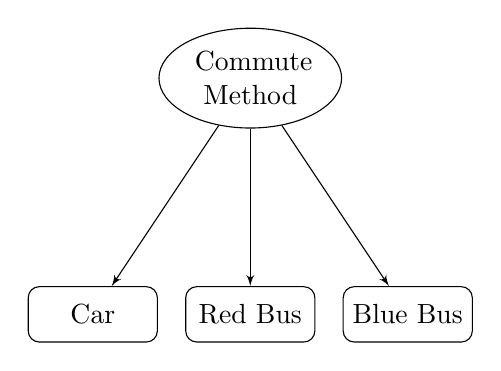
\begin{tikzpicture}[node distance=2.5cm, auto]
    \node [decision] (commute) {Commute Method};
    \node [process, below of=commute, xshift=-2cm] (car) {Car};
    \node [process, below of=commute             ] (redbus) {Red Bus};
    \node [process, below of=commute, xshift= 2cm] (bluebus) {Blue Bus};
    
    \path [line] (commute) -- (car);
    \path [line] (commute) -- (redbus);
    \path [line] (commute) -- (bluebus);
\end{tikzpicture}
\end{center}
}

\end{frame}

\begin{frame}

\onslide<1->{
One way to get around IIA is to \textcolor{hi}{nest} the choice set
}

\bigskip{}

\onslide<2->{
Nesting maintains IIA at each level but breaks IIA across alternatives in different nests
}

\bigskip{}

\onslide<3->{
\begin{center}
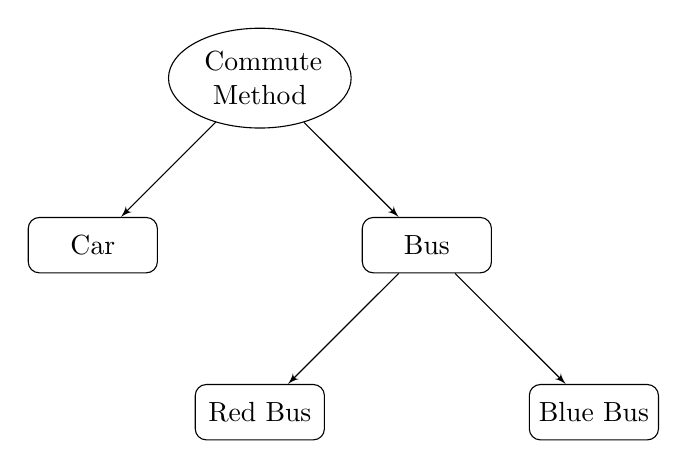
\begin{tikzpicture}[node distance=2.5cm, auto]
    \node [decision] (commute) {Commute Method};
    \node [process, below left of=commute] (car) {Car};
    \node [process, below right of=commute] (bus) {Bus};
    \node [process, below left of=bus] (redbus) {Red Bus};
    \node [process, below right of=bus] (bluebus) {Blue Bus};
    
    \path [line] (commute) -- (car);
    \path [line] (commute) -- (bus);
    \path [line] (bus) -- (redbus);
    \path [line] (bus) -- (bluebus);
\end{tikzpicture}
\end{center}
}

\end{frame}

\end{document}